\documentclass{llncs}

%\usepackage{makeidx}  % allows for indexgeneration
\usepackage{graphicx}

\begin{document}

\title{Mailing lists meet the Semantic Web}

\titlerunning{Mailing lists meet the Semantic Web}

\author{
Sergio Fern\'andez\inst{1} \and Diego Berrueta\inst{1} \and Jose E. Labra\inst{2}
}

\authorrunning{Sergio Fern\'andez et al.}

\tocauthor{Sergio Fern\'andez, Diego Berrueta, Jose E. Labra} 

\institute{%
Fundaci\'on CTIC, \\
Gij\'on, Asturias, Spain,\\
\email{\{sergio.fernandez,diego.berrueta\}@fundacionctic.org}
\and
Universidad de Oviedo,\\
Computer Science Department,\\
Oviedo, Asturias, Spain,\\
\email{labra@uniovi.es}\\
}

\date{18 February 2007}

\maketitle

\begin{abstract}

Mailing list archives (i.e., the messages posted up-to-now) are often published 
on the web and indexed by conventional search engines. They store a vast 
knowledge capital. However, the ability to auto-matically recognize and process 
the information is mostly lost at publishing time. As a result, the current 
mailing list archives are hard to query and have a limited use. This paper 
describes how SWAML uses Semantic Web technologies in order to avoid the
information loss and to allow new applications able to exploit this 
information in a more convenient way.

\end{abstract}

\section{Introduction}

Electronic mail (e-mail) remains one of the most
popular applications of the Internet. Besides direct messaging
between individuals, mailing lists exist as private or public
forums for information exchange in communities with shared interests.
Mailing list archives are compilations of the previously posted
messages that are often converted into static HTML for its
publication on the web. They represent a significative portion of
the contents that are indexed by the web search engines, and they
capture an impressive body of knowledge that, however, is difficult
to locate and browse.

The root of these problems can be traced back to the translation
procedure that is run to transform the e-mail messages into static
HTML pages. This task is fulfilled by scripts that create an
static HTML page for each message in the archive, in addition to
some indexes (by date, by author, by thread), often splitted by
date intervals to avoid excessive growth. On one hand, this fixed
structure reduces the flexibility when the user browses the
mailing list archives from his web browser. On the other one, some of
the metadata that was associated to each e-mail message is lost
when it is rendered as HTML for presentational purpouses.

We propose to use an ontology and RDF to enable the publishing of
the mailing list archives into the (Semantic) web, while retaining
the metadata that were present in the messages. The rest of the
paper is organized as follows: Section~\ref{sec:SIOC} introduces the
SIOC ontology and our extensions to it, and then our software
applications are described in Section~\ref{sec:software}. We close
the paper with the conclussions and a discussion on our future plans
in Section~\ref{sec:conclussions}.

\section{\label{sec:SIOC}SIOC}

SIOC (Semantically-Interlinked Online Communities) provides methods for 
interconnecting discussion methods such as blogs, forums and mailing lists 
to each other. It consists of the SIOC ontology, an open-standard machine 
readable format for expressing the information contained both explicitly 
and implicitly in internet discussion methods, of SIOC metadata producers 
for a number of popular blogging platforms and content management systems, 
and of storage and browsing/searching systems for leveraging this SIOC 
data~\cite{Breslin2005}.

The goal of SIOC \footnote{\url{http://sioc-project.org/}} is to interconnect
these online communities. Community sites can include many discussion primitives,
such as bulletin boards, weblogs and mailing lists, which it have grouped under 
the concept of forum.

%\begin{figure}[ht]
% \centering
% 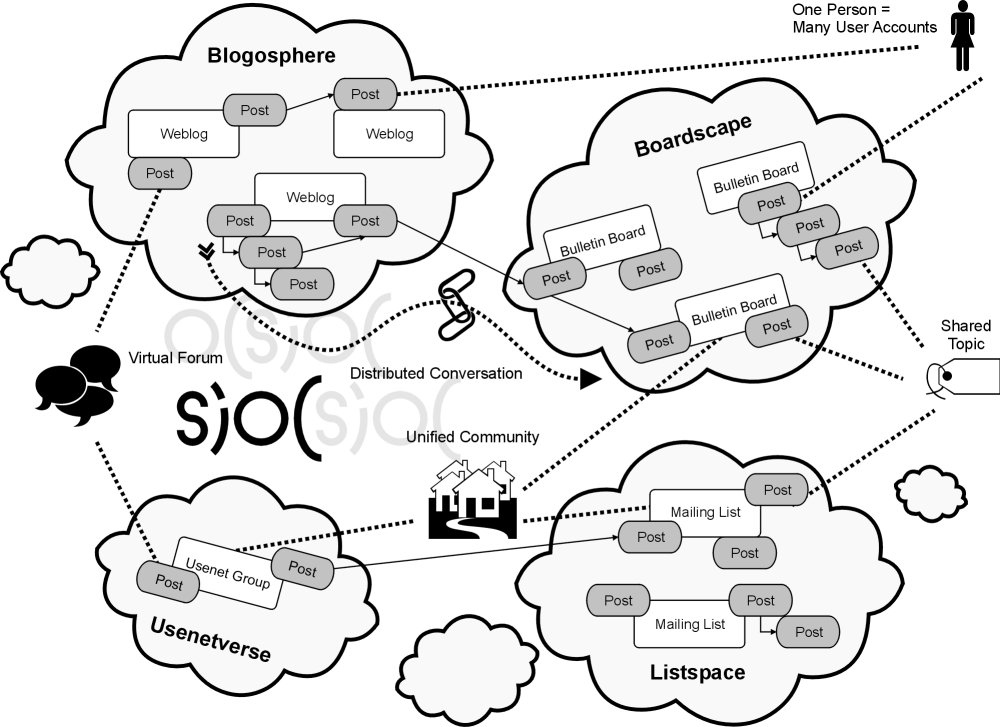
\includegraphics[bb=0 0 240 174]{images/sioc-discussion.png}
% \caption{Connections between discussion clouds with SIOC}
%\end{figure}

FIXME: add a graphic about relations between forums

Then \texttt{Forum} class is the most important for us at SIOC ontology. In the 
domain of a forum there are another classes at the ontology, mainly we need two
of it: \texttt{Post} and \texttt{User} 

The SIOC community has developed several wrappers that allows to export instances
of community site concepts (such as blogs o forums) in RDF format. But the effort 
is only centered in providing mappings from web-based systems, forgetting all the 
knowledgement stored in a large number of legacy systems preceding the current Web.

\subsection{Our extension}

Until SIOC ontology contemplates some subclasses of Forum, it's necessary 
to add some properties. Concretely in version 0.2 of our ontology 
\footnote{http://swaml.berlios.de/ns/0.2} we have reduced these properties 
to only two:

\begin{itemize}
  \item \texttt{previousByDate} to link with the previous post sent in the 
	mailing list..
  \item \texttt{nextByDate} to link with the post that was sent after by date 
	in the mailing list.
\end{itemize}

Both under the domain and the range of \texttt{sioc:Post}. Perhaps these 
properties has a minor importance to describe generic forums instances, 
but its meaning receives greater importance in the concrete scope of a 
mailing list.

\section{\label{sec:tools}Software tools}

In the SWAML project ahas been developed some software tools, mainly three:

\begin{itemize}
 \item SWAML, the core process that exports a mailing list in RDF.
 \item Buxon, a browser for SIOC Forum instances.
\end{itemize}

Each of it each one fulfills a concrete purpose into the global purposes that 
the project persecutes. The project covers so much the data exportation phase 
as the data consumition phase.

\subsection{SWAML}

The main component, the core, is called with the same name that the project. SWAML is
the process in charge to process the mailing lists. SWAML reads a collection of email 
messages stored in a mailbox (from a mailing list compatible with RFC 4155) and generates 
a RDF description. It is written in Python using SIOC as the main ontology to represent 
in RDF a mailing list.

\begin{figure}[ht]
 \centering
 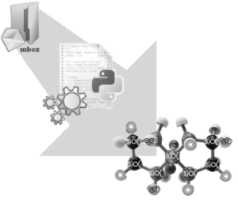
\includegraphics[bb=0 0 238 200]{images/swaml-process.png}
 \caption{SWAML core process}
\end{figure}

The SWAML project fulfills a much-needed requirement for the Semantic Web: to be able 
to refer to semantic versions of email messages and their properties using a resource 
URI. By reusing the SIOC vocabulary for describing online discussions, SWAML allows 
users of SIOC to refer to email messages from other discussions taking place on forums, 
blogs, etc., so that distributed conversations can occur across these discussion media. 
Also, by providing email messages in SIOC format, SWAML are providing a rich source of 
data, namely mailing lists, for use in SIOC applications.

But this component not only exports a mailbox, it goes a little more far...

Firstly it tries to find a FOAF profile that describes a person with the mail address 
of each subscriber. This it isn't a trivial task with the infrastructure of the actual 
Semantic Web, because there isn't any service that provides this specific functionality.
For the moment this part is only a mock, but it's ready to work when we'll finish another 
project.

Secondly it exports all the geographical information found in these FOAF profiles into 
KML~\cite{KML}, to draw the point into Google Maps or Google Earth.

\begin{figure}[ht]
 \centering
 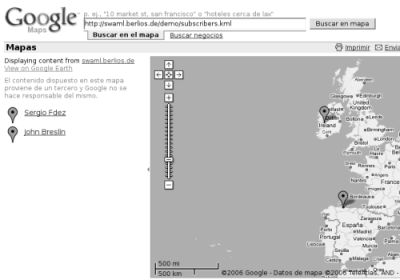
\includegraphics[bb=0 0 400 280]{images/googlemaps.png}
 %FIXME: add a screeshot with more points
 \caption{Subscribers' geographical information on Google Maps}
\end{figure}

\subsection{Buxon}

Buxon is the application that make the opposite work. It takes the URI of a generic SIOC 
Forum (for example a mailing list exported by SWAML, although it's independent of the 
export tool) and it recompose the graph. With that graph the tool shows the posts ordered 
by threads using a similar GUI than the classic mail clients.

\begin{figure}[ht]
 \centering
 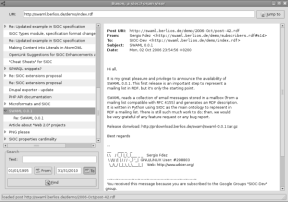
\includegraphics[bb=0 0 288 202]{images/buxon.png}
 \caption{Buxon in action (FIXME: add a screenshot of v0.0.4)}
\end{figure}

In addition it allows to make simple searches by terms and dates over the back-end graph.

FIXME: support to PingTheSemanticWeb.com (search a cite)

\section{\label{sec:conclussions}Conclussions and Future Work}

There is a lot of ongoing effort to translate data already reachable
on the web into formats
which are Semantic Web-friendly. Most of that work focuses on relational
databases, microformats and web services. However, at the time of this
writing and to the best of our knowledge, e-mail was almost excluded from the
Semantic Web. This project, in combination with the generic SIOC framework,
fills this gap, conveniently providing
an ontology and a parser to publish machine-readable versions of the
archives of the countless mailing lists.

Some benefits arouse from the availability of these data. In the first
place, data can be fetched by user applications to provide handy browsing
through the archives of the mailing lists, providing features that
exceed what is now offered by static HTML versions of the archives on
the web.

Secondly, the bot crawlers of the web search engines can use the enhanced
expressivity of the RDF data to refine search results. For instance, it
becomes possible to filter out repeated messages, advance in the fight against
spam, or introduce additional filter criteria in the search forms.

Another consequence of no lesser importance is that each e-mail message
is assigned a URI that can be resolved to a machine-readable description
of the message. This actually makes possible to link a message like
any other web resource, and therefore enriches the expressivity of the
web.

We are exploring some directions for future work. Some of them are:

\begin{itemize}
  \item Integration of the SWAML process with a popular HTML-based
        mailing list archiver, such as Hypermail or Pipermail, would be
        a gigant push to speed up the adoption of SWAML. It is well
        known that one of the most awkward problems of any technology
        is to gain a critical mass of users. The semantic web is not
        an exception. A good recipe to tackle this problem is to
        integrate the new technologies into old tools, making
        a smooth transition without requiring any extra effort from
        the users. Merging the SWAML process into the batch flow of
        tools such as Hypermail would allow to generate both
        HTML and RDF versions of the archive. Those could reside
        side-by-side on the web server, even sharing the same URI
        by means of content-negotiation~\cite{Recipes}.
  \item Actually, integration could be pushed further away through
        RDFa~\cite{Birbeck2006}, embedding the RDF content into the
        XHTML documents.
  \item So far, no semantic annotation relative to the meaning of
        the messages is considered. Obviously, this information can not
        be derived from a RFC 4155-compilant mailbox\cite{RFC4155}.
        However, it is
        conceivable that it can be added by other means, for instance,
        by social tagging using folksonomies, or by parsing the RDFa
        that can exist in the messages that are send in XHTML format.
  \item The metadata extracted from a mailing list archive can be
        quite huge. Even after removing the body of the messages, the
        XML/RDF metadata of a mailing list containing 1000 messages may
        have a size of 4 MBytes, with a linear growth. It is not uncommon
        for a busy mailing list to generate this volume of messages
        monthly. Hence, it is imperative to design a mechanism to
        fragmentate the dataset. The SWAML process splits each message
        in a separate RDF document, but this arbitrary decision clearly
        does not fit every application. A much better solution would be to
        create an easy-to-deploy SPARQL endpoint~\cite{SPARQLProtocol},
        that translates the
        decision on how to partition the data to the final application.
  \item It is not always possible to obtain a mailbox file for a mailing
        list. For these cases, an alternative is envisaged: a high-capacity
        GMail account can be subscribed to the mailing list with the unique
        purpose of collecting and storing the messages. A simple extension
        to SWAML that makes possible to import the contents of a GMail
        account has been developed.

\end{itemize}

\section*{Acknowledgements}

The authors would like to express their gratitude to Dr. John Breslin and
Uldis Bojars from DERI Galway, whose support and contributions have been of 
great help to this project.

\bibliographystyle{abbrv}
\bibliography{../references}
%
\end{document}
